\documentclass[12pt, letterpaper, titlepage]{article}

\usepackage{amsmath}
\usepackage{booktabs}
\usepackage{amsthm}
\usepackage{graphicx}
\usepackage[margin=1in]{geometry}
\usepackage{hyperref}
\hypersetup{colorlinks = true, linkcolor = blue, citecolor=blue, urlcolor = blue}
\usepackage{natbib}
\usepackage{enumitem}
\usepackage{setspace}

\usepackage[pagewise]{lineno}
%\linenumbers*[1]
% %% patches to make lineno work better with amsmath
\newcommand*\patchAmsMathEnvironmentForLineno[1]{%
 \expandafter\let\csname old#1\expandafter\endcsname\csname #1\endcsname
 \expandafter\let\csname oldend#1\expandafter\endcsname\csname end#1\endcsname
 \renewenvironment{#1}%
 {\linenomath\csname old#1\endcsname}%
 {\csname oldend#1\endcsname\endlinenomath}}%
\newcommand*\patchBothAmsMathEnvironmentsForLineno[1]{%
 \patchAmsMathEnvironmentForLineno{#1}%
 \patchAmsMathEnvironmentForLineno{#1*}}%

\AtBeginDocument{%
 \patchBothAmsMathEnvironmentsForLineno{equation}%
 \patchBothAmsMathEnvironmentsForLineno{align}%
 \patchBothAmsMathEnvironmentsForLineno{flalign}%
 \patchBothAmsMathEnvironmentsForLineno{alignat}%
 \patchBothAmsMathEnvironmentsForLineno{gather}%
 \patchBothAmsMathEnvironmentsForLineno{multline}%
}

% control floats
\renewcommand\floatpagefraction{.9}
\renewcommand\topfraction{.9}
\renewcommand\bottomfraction{.9}
\renewcommand\textfraction{.1}
\setcounter{totalnumber}{50}
\setcounter{topnumber}{50}
\setcounter{bottomnumber}{50}

\newcommand{\jy}[1]{\textcolor{blue}{JY: #1}}
\newcommand{\eds}[1]{\textcolor{red}{EDS: (#1)}}


\title{Time Series Length at Which Block Bootstrapping is Effective for Estimation of Variance}

\author{Mathew Chandy\\
%   \href{mailto:mathew.chandy@uconn.edu}
% {\nolinkurl{mathew.chandy@uconn.edu}}\\
  Jun Yan\\[1ex]
  Department of Statistics, University of Connecticut\\
}
\date{}

\begin{document} 
\maketitle

\doublespace

\begin{abstract}
Block bootstrapping is a method that can be used for estimating a statistic of a time
series. It involves splitting a series into blocks (in order to account for the time
factor) and re-sampling the blocks to create many new bootstrapped time series.
This method becomes more effective as the length of the time series increases. 
The question for this study is how does one determine at what length the block
bootstrap method stops being an effective method to estimate a statistic of a time
series.

\bigskip
\noindent\sc{Keywords}:
block bootstrap;
\end{abstract}

\section{Introduction}
\label{sec:intro}

Block bootstrapping is a widely used method in Statistics. The concept for block 
bootstrapping was developed independently by \citet{hall1985resampling}, \citet{carlstein1986use}, and 
\citet{kunsch1989jackknife}. \citet{radovanov2014comparison} It has been applied to a variety of 
different fields such 
as econometrics \citep{mackinnon2006bootstrap} and meteorology \citep{varga2017generalised}. It can be used for 
situations in which there is temporal dependence and the goal is estimation or hypothesis 
testing. Assuming that the sample is infinitely 
large, the method will work perfectly. However, for a finite sample size, the method will 
not work as well as expected. It may be necessary (in order to plan an applied 
statistical 
procedure) to know at which sample size the method stops working at an acceptable level. 
The goal of this study is to find a threshold or range of sample sizes at block bootstrap 
is no longer an effective method for estimating variance.


\citet{nevitt2001performance} find that a sample size of 200-1000 is usually sufficient for standard 
bootstrap estimation. However, block bootstrapping is a different situation because the 
sample is split into blocks.

\citet{goncalves2005bootstrap} found that standard error estimates from block bootstrapping small 
samples 
may be significantly more accurate than inference from closed-form asymptotic estimates. That study focused on variance estimation within the context of linear regression. Still, the rate at which confidence intervals recover the true variance for small sample sizes wasn't very close to the confidence level of the intervals. This study aims to find how small the sample size can be for time series (which has a dependence factor which can be compared to a linear regression) in order for the coverage rate to be close to the confidence level.

For this study, many block bootstrap simulations were conducted with R. At the base
level, we are block-bootstrapping an auto-regressive process with true mean 0.
Bootstrapping is the term for creating new samples of the same size by re-sampling from
the original sample with replacement. Many bootstrapped samples are used to create a
distribution of sampling means to estimate mean and variance. This works for samples
that are not dependent. However, for a time series such as an auto-regressive process,
a different procedure is required to account for the time dependence. In such a case,
the series is split into blocks that may overlap (moving block bootstrap) or may not
overlap (non-moving block bootstrap). These blocks are then re-sampled to create new
bootstrapped time series. 

In our experiment, we find the means of a 1000 block-bootstrapped time series, 
and create a 95 \% confidence interval of the means. We replicate this 1000 times, 
and record the proportion of confidence intervals that recover the true mean 
(coverage rate). We are effectively observing how successful the bootstrapping process
is at estimating the mean and variance. The key variable being observed was n, 
the length of the time series, or the size of the sample. It is known that as n
increases, block bootstrapping will become a less accurate method for estimation
(the coverage rates will decrease). The question is at what range of n values does this
start to become a problem. 

In this experiment, there are certain factors that are expected to affect the coverage
rates. As the Auto-Regressive (AR) coefficient (the time dependence) of the time series 
increases,
we expect the coverage rates of the confidence intervals to decrease.
The coverage rates are also affected by the size of the blocks - more specifically,
how the size of the blocks (l) relates to the size of the time series (n) - 
and whether or not they overlap. It is known that as the size of the time series 
increases, the optimal block length should increase, and the ratio of the block length to 
the time series length should decrease. l = n$^3$ is typically considered the optimal 
block length according to asymptotic theory. \citep{buhlmann1999block} If only perfect cubes are used for the time 
series length, n gets too large when l increases by relatively little. An alternative 
would be to use smaller time series, find the cube root, and set the block length to the 
nearest whole number. However, in this study l = sqrt{n} is used, as it allows for smaller 
sample sizes, but it still follows the aforementioned principle.

So to solve the question of what n is necessary for effective block bootstrapping,
while still accounting for all these factors, the simulations were repeated for
multiple combinations of AR coefficient and the function of n used to decide l. In 
addition, the coverage rates
for both the non-moving and moving methods were recorded.

\section{Review of Block Bootstrap}
\label{sec:blkbootreview}

Block bootstrapping is a method that can be applied to time series to estimate a parameter and it's variance. Suppose that a sample of size n of a time series is given. In order to account for the temporal dependence, the time series can be split into blocks, typically of the same size. The block should be of size l large enough to include time dependence, yet small enough to include some variance. The designer of the study can choose whether the blocks overlap or not. If the bloc(Figure here) A bootstrapped sample is created by taking a sample of n / l blocks with replacement to create a new series of size n. An estimator of the parameter is computed from the sample. This procedure can be repeated many times to create a sampling distribution if the distribution is unknown. Using this sampling distribution, a confidence interval for the parameter can be created using the alpha/2 and 1 - alpha/2 percentiles.



\section{Simulation Study Design}
\label{sec:simdesign}

The basic objective of the study was to assess how well block bootstrap estimates the variance for an autoregressive process. In the previous section, the process for creating a confidence interval using the block bootstrap method is described. This process is applied to a simulation of an autoregressive integrated moving average (ARIMA) with sigma = 0.1 to create a confidence interval of the mean of the process. For a certain AR coefficient, a block bootstrap 95\% confidence interval is replicated 1000 times at a starting sample size at which block bootstrap is expected to be very effective. For each individual confidence interval, it can be recorded whether or not the interval includes the true mean (0). The coverage rate, or the proportion of intervals that include the mean, can then be recorded. If the variance is being properly estimated by the block bootstrap, the coverage rate should reflect this by being close to the confidence level of 95\%. If this is not the case, the method is not working as well as it should. Since the coverage rate is a proportion, a 95\% confidence interval of the coverage rate can also be created.





\section{Methods}
\label{sec:methods}

Before each simulation, the random seed was set to 5 so that the randomized results can be 
reproduced. 

A simulation of an autoregressive integrated moving average (ARIMA) process was run 
repeatedly with varying parameters. 
The mean and standard deviation of the time series was held constant at 0 and 0.1, whereas 
the sample size and AR Coefficient
 were varied. The AR Coefficients that were used were 0.2, 0.4, and 0.6. The sample sizes 
 that were used depended on the AR
 Coefficient, and the function used to compute l. For each of these variations, 1000 
 confidence intervals are created using
 the block bootstrap method, and the proportion of these intervals that recover the true 
 mean (0) is recorded as the coverage
 rate. The block bootstrap method has different settings that were varied in this study: 
 non-moving vs moving, 
and the function for block length - the two used were a constant block length of 10 and 
the square root of n.

For the simulations using a constant block length of 10, the sample size was gradually 
lowered by increments of 20 to see when
the block bootstrap would begin to consistently return low coverage rates. For AR = 0.2 
using a constant l, results for
sample sizes ranging from 400 to 20 were observed. For AR = 0.4 using a constant l, 
results for sample sizes ranging from 600
to 20 were observed. For AR = 0.6, using a constant l, results for sample sizes ranging 
from 900 to 120 were observed. For the simulations in which the block length was the 
square root of the time series length, the only sample sizes used were perfect squares so 
that the blocks would have whole number lengths. For AR = 0.2 using l = sqrt{n}, results 
for sample sizes ranging from 625 to 36 were observed. For AR = 0.4 using sqrt{n}, results 
for sample sizes ranging from 900 to 121 were observed. For AR = 0.6 using l = sqrt{n}, 
results for sample sizes ranging from 1600 to 121 were observed. 

\section{Results}
\label{sec:results}

As the AR Coefficient increases, it was found unsurprisingly that a larger sample size was 
required for effective block bootstrap estimation. 



\begin{figure}[tbp]
  \centering
  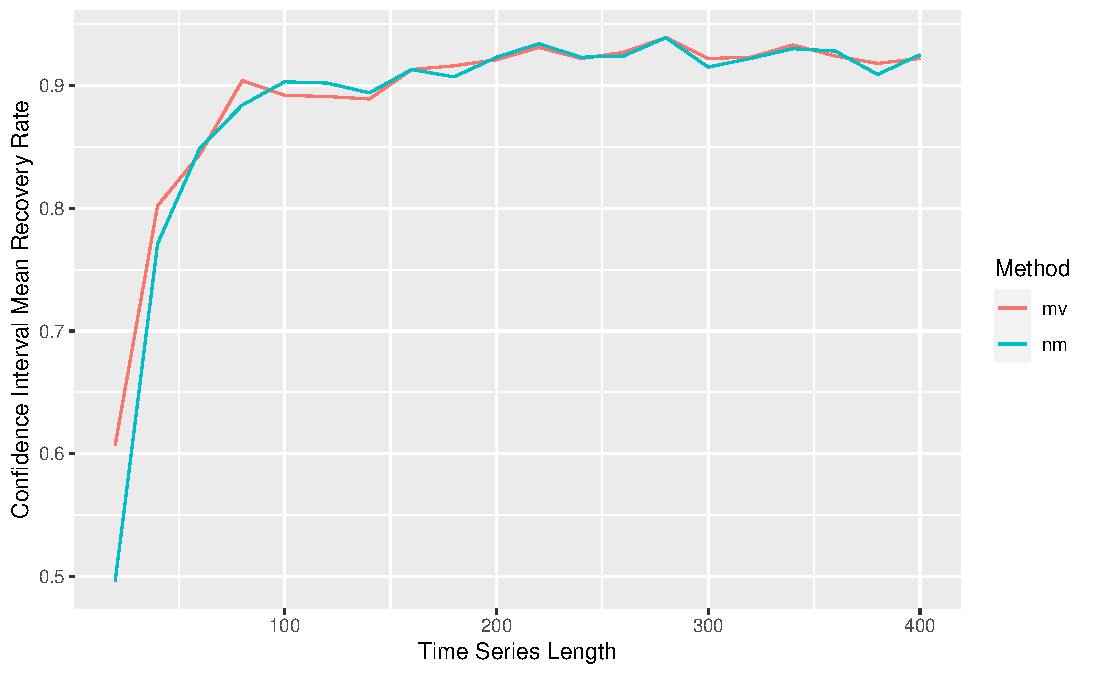
\includegraphics[width=\textwidth]{constant_0.2}
  \caption{}
  \label{fig:constant_0.2}
\end{figure}

\begin{figure}[tbp]
  \centering
  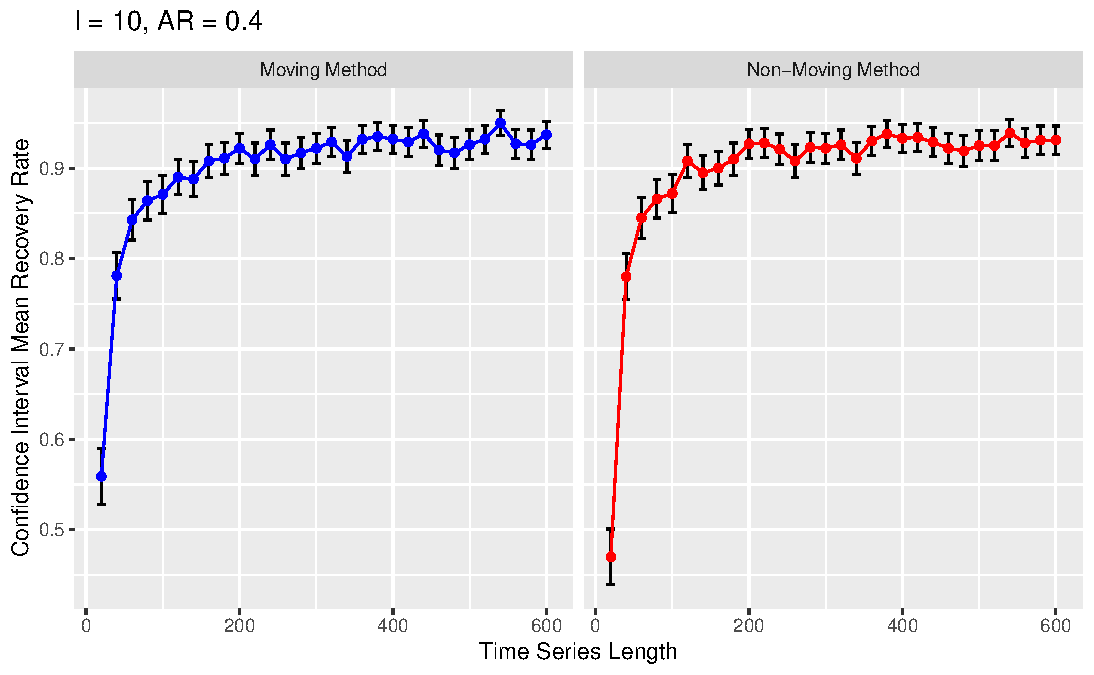
\includegraphics[width=\textwidth]{constant_0.4}
  \caption{}
  \label{fig:constant_0.4}
\end{figure}

\begin{figure}[tbp]
  \centering
  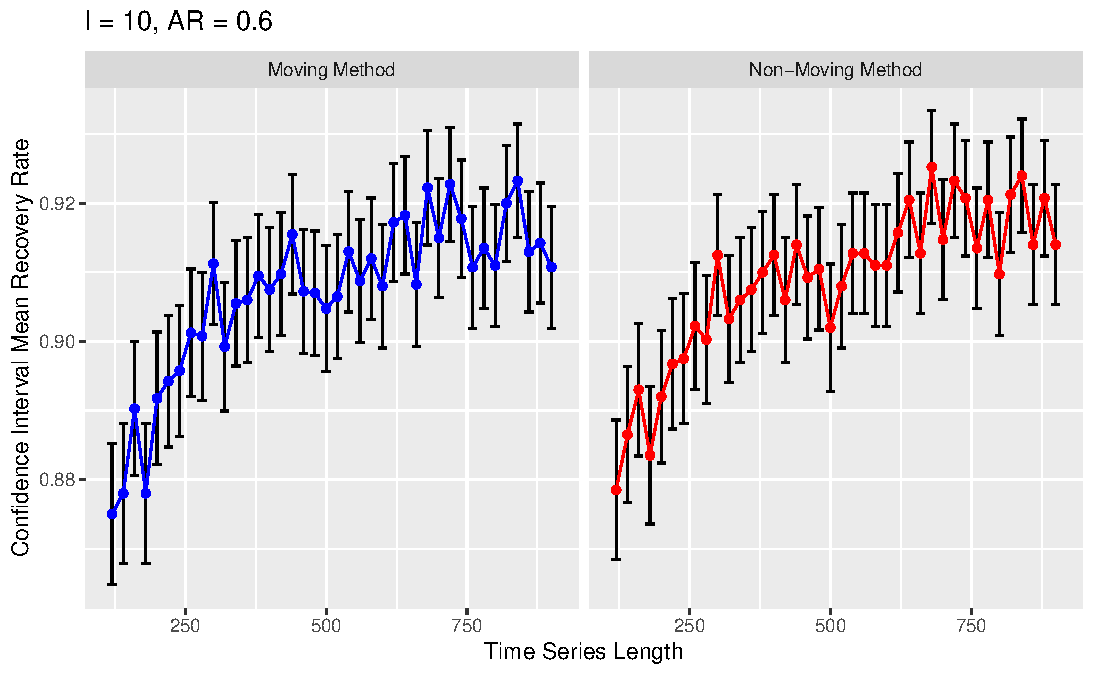
\includegraphics[width=\textwidth]{constant_0.6}
  \caption{}
  \label{fig:constant_0.6}
\end{figure}

\begin{figure}[tbp]
  \centering
  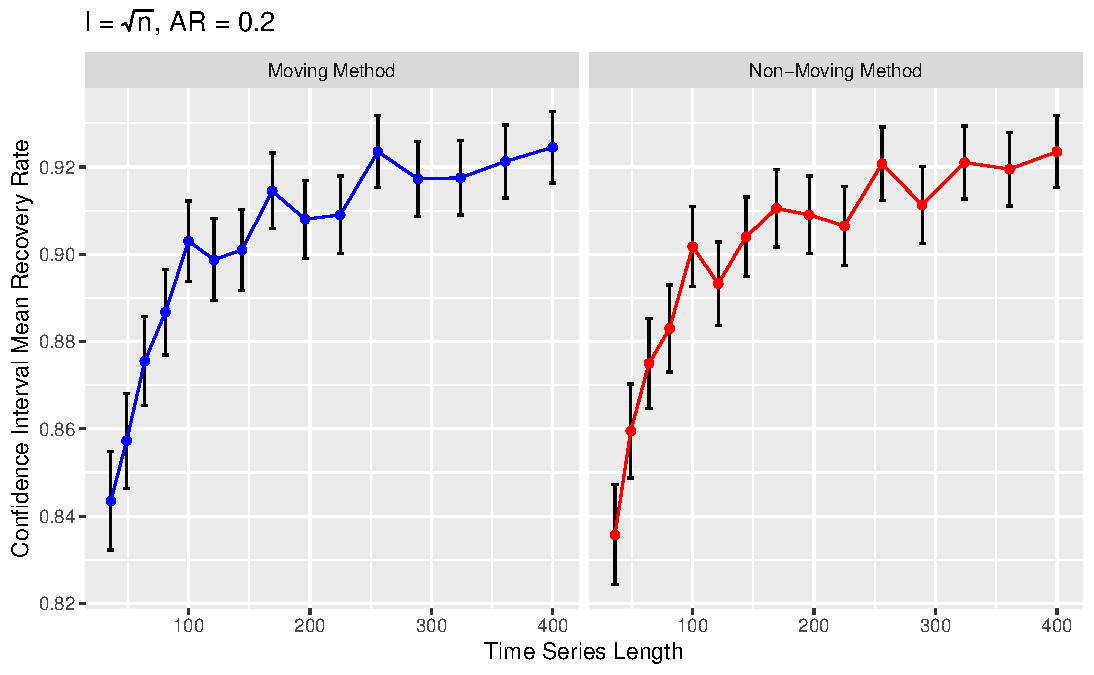
\includegraphics[width=\textwidth]{root_0.2}
  \caption{}
  \label{fig:root_0.2}
\end{figure}

\begin{figure}[tbp]
  \centering
  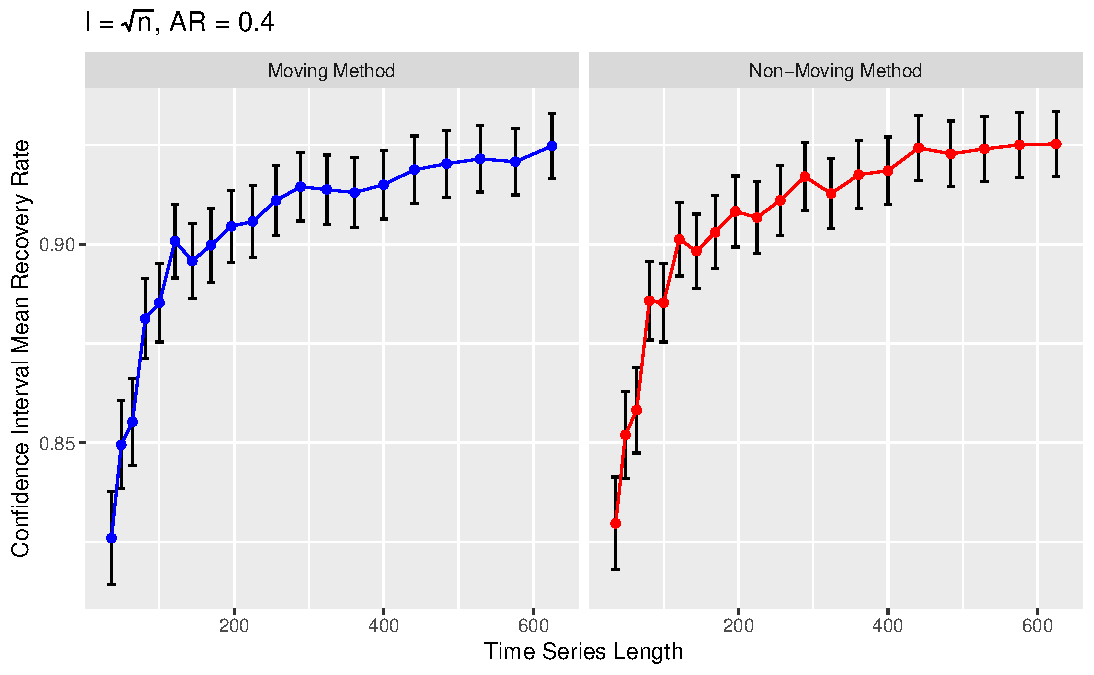
\includegraphics[width=\textwidth]{root_0.4}
  \caption{}
  \label{fig:root_0.4}
\end{figure}

\begin{figure}[tbp]
  \centering
  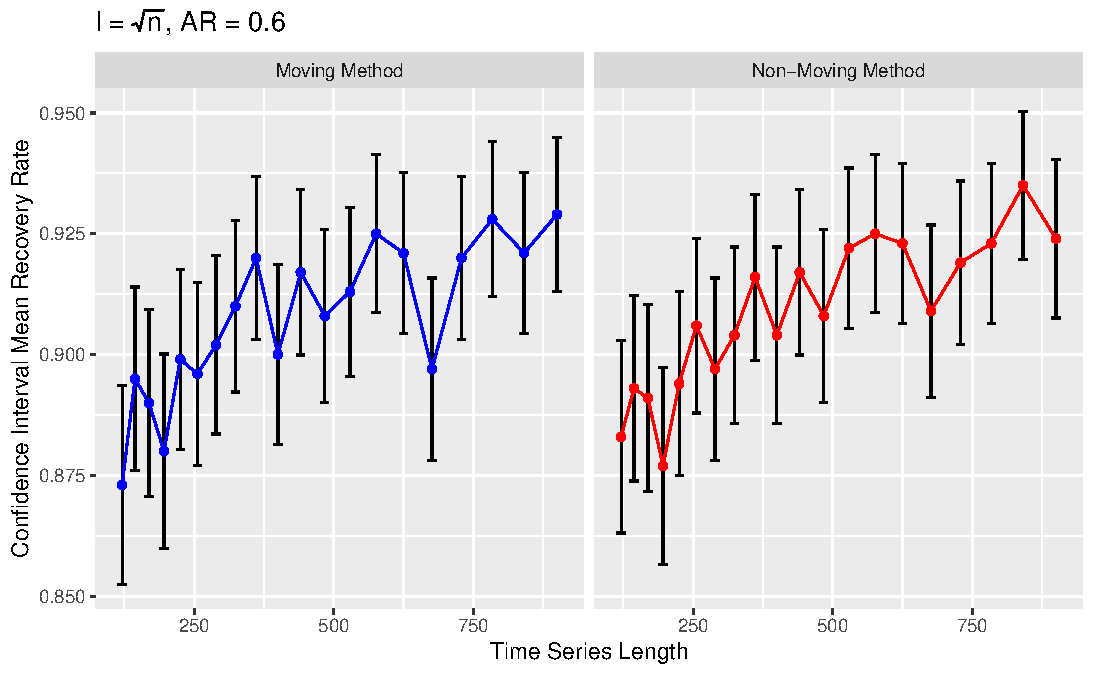
\includegraphics[width=\textwidth]{root_0.6}
  \caption{}
  \label{fig:root_0.6}
\end{figure}

\label{sec:results}




\section{Discussion}
\label{sec:discuss}



\bibliographystyle{chicago}
\bibliography{citations.bib}


\end{document}